\chapter{Delitos informáticos en Chile}
\section{Casos a nivel nacional}

\subsection{Hackeo a Fuerza aerea}
Hackers peruanos intervinieron los correos electronicos de la FACH liberando cientos de correos electrónicos de la institución militar, con información privada de funcionarios, de sus familias y de la Administración de Contratos del Comando de Logística.

Los mensajes contenían información de varias negociaciones y contratos de la FACH para la compra de misiles, sistemas de radares, aviones y otros implementos. Entre ellas, compra de armamento estratégico a la empresa israelí de defensa Rafael Advanced Defense System Ltd. y a otra francesa.

Se descarto según la entidad que se haya puesto en peligro la seguridad nacional de Chile. Además, precisaron que el ataque se produjo entre mayo y junio de 2013 y que tras lo sucedido implementaron un nuevo sistema de correos electrónicos con mayor seguridad.\cite{aerea}

\subsection{Hackeo pagina web de gobierno}
Un niño de 12 años, residente de Montreal, Canadá, se declaró culpable de tres cargos de 'hackeo' de páginas web gubernamentales, entre ellas la de la Policía de Montreal, el Instituto de Salud Pública de Quebec y del Gobierno de Chile, en 2012.
Los ataques tuvieron lugar durante las protestas estudiantiles en Canadá y fueron realizados bajo la iniciativa de los 'hacktavistas' de Anonymous. Se trató de asaltos de tres tipos, incluidos los ataques DoS, cuando un objetivo es bombardeado con solicitudes destinadas a consumir gran parte de sus recursos para que se vuelva inaccesible a los usuarios legítimos.\cite{nino}

\subsection{Hackeo pagina web de Ministerio de Defensa}
La página web del Ministerio de Defensa de Chile fue hackeada y se mostraron mensajes alusivos al grupo terrorista Estado Islámico como se ve en la figura 
~\ref{fig:hackmin}.
El Ministerio de Defensa dijo en un comunicado que el ataque “no puso en riesgo información sensible ni sus correos electrónicos”.
Igualmente dijo que se abrió una investigación para identificar el origen de los hechos que quedo en nada. En tanto, la página fue redirigida temporalmente a otra unidad del Ministerio para luego ser restablecida.
\begin{figure}[H]
\label{fig:hackmin}
\centering
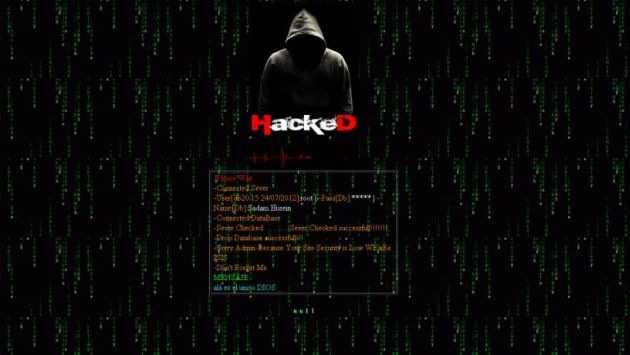
\includegraphics[width=\textwidth]{img/ministeriohack.jpg}
\caption{Imagen al momento que fue hackeada la pagina del ministerio de defensa}
\label{fig:diagrama01}
\end{figure}
\subsection{Tarjeta BIP}
La aplicación permite que un smartphone con NFC sea capaz de recargar una tarjeta Bip! sin pago alguno, saldo que luego es reconocido como válido por los 'totems' (las máquinas que leen el saldo de la tarjeta).
El fraude se llevó a cabo a partir una aplicación para teléfonos Android y a través de la tecnología de comunicación inalámbrica de corto alcance (NFC, por sus siglas en inglés) incorporada en el smartphone del usuario.\cite{bip}
De acuerdo al análisis realizado, el proceso de recarga gratuita era muy sencillo. El usuario sólo necesitaba descargar la aplicación en un dispositivo Android capacitado para usar tecnología NFC, acercar la tarjeta de viaje al teléfono y presionar el botón Cargar 10k, lo que les permite recargar la tarjeta con 10 mil pesos. Ver figura ~\ref{fig:hackvip}.
\begin{figure}[H]
\label{fig:hackvip}
\centering
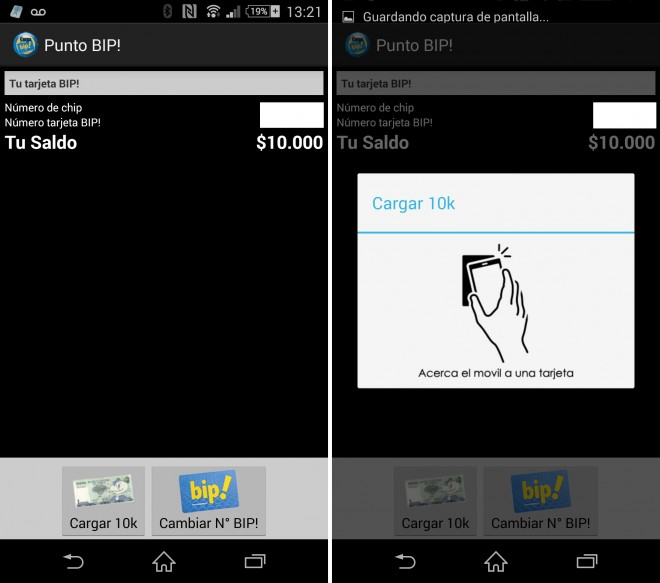
\includegraphics[width=\textwidth]{img/hackvip.jpg}
\caption{Interfaz gráfica de la aplicación maliciosa de recarga de tarjetas Bip!}
\label{fig:diagrama01}
\end{figure}

\subsection{Pishing en Chile}

\subsubsection{Banco Chile}
Hace un par de años sufrió de Pishing hacia sus clientes, de alguna manera los atacantes obtuvieron un gran listado de clientes donde por medio de un correo electrónico se le solicitaban ingresar datos privados de sus cuentas bancarias.. 

La vista de este ataque de suplantación de identidad lo podemos ver en la figura ~\ref{fig:banchile}
\begin{figure}[H]
\label{fig:banchile}
\centering
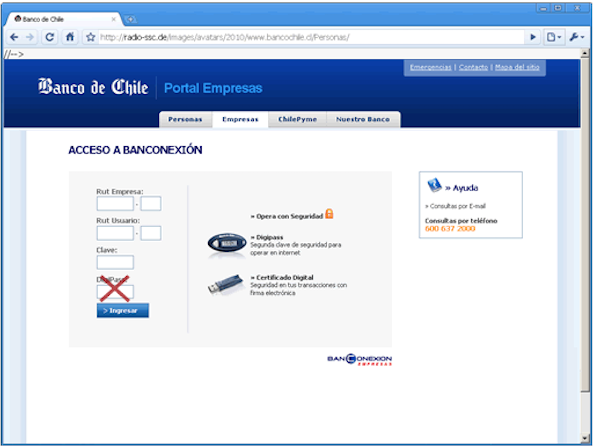
\includegraphics[width=\textwidth]{img/banco.png}
\caption{Vista de la falsa URL dada por los atacantes via correo electronico}
\label{fig:diagrama01}
\end{figure}

\subsubsection{Delincuencia y el Pishing}
Los delincuentes utilizan este método para captar los antecedentes bancarios de los afectados, o sea, crear falsas páginas de bancos como en el caso anterior, por las que pedía cambiar las contraseñas y otros datos, y que eran enviadas a potenciales víctimas.

Luego, realizan las compras a través de los portales. Pero las especies no llegaban a su casa, sino que a las de otras personas quienes reciben un porcentaje de ganancia.\cite{flaite}

Por lo general son delincuentes sin mucho conocimiento informático o están dentro de cárceles realizando los delitos, a pesar de casos particulares por lo general esta estafa es fácil de detectar debido a la poca credibilidad que generan sus correos para captar víctimas.

\section{Impacto en el país}
Si se encuentran vulnerabilidades y estás son explotadas pueden generar un gran daño o un aprovechamiento exagerado de estas como tenemos el caso de cuando a mediados de octubre del 2014 un grupo de informáticos logro hackear la tarjeta BIP del transporte público del país donde ingresaban dinero a la tarjeta bip sin gastar de su bolsillo, esto genero grandes gastos para el transporte público siendo que es una de las áreas donde el gobierno siempre inyecta dinero para mejorarlo esto genera un retroceso en su presupuesto por la evasión generada por estas tarjetas BIP hackeadas, es decir un impacto monetario. 

Se pueden generar impactos a nivel de confidencialidad, si por ejemplo sucediera un robó información escencial para el Estado de Chile, por ejemplo militar, y cae en manos equivocados dicha información puede traer como consecuencias vulnerabilidades dispuestas a ser explotadas por algún presunto enemigo. 
% Alejandro Vega para de mentir volao ctm 
% Felipe Rios el falloo más mentiroso
